\documentclass{article}
\usepackage[margin=1in]{geometry}
\usepackage{amsmath}
\usepackage{graphicx}


\begin{document}

\title{\textbf{Tail Sizing}}
\author{Abigail Gries}
\maketitle

The tail of an aircraft or UAS is key in providing stability, control, and trim. In order to correctly size the tail for the OpenUAS, the center of gravity must first be located. This document describes the process for determing the center of gravity and how to use that information to determine the appropriate surface areas for the horizontal and vertical tails. This document also explains which airfoil the OpenUAS team chose for the tail and provides a brief overview of that airfoil's characteristics. 

\section*{Variables}
\textit{b} = wingspan \\
$\bar{c}$ = mean chord length \\
\textit{cg} = preliminary center of gravity \\
%$cg_{HT}$ = aerodynamic center of gravity of horizontal tail \\
%$cg_{VT}$ = aerodynamic center of gravity of vertical tail \\
\textit{d} = moment arm \\
$l_{HT}$ = horizontal distance between the center of gravity and the aerodynamic center of horizontal tail \\
$l_{VT}$ = vertical distance between the center of gravity and the aerodynamic center of vertical tail \\
$M_N$ = moment about the nose \\
\textit{S} = wing surface area \\
$S_{HT}$ = horizontal tail surface area \\
$S_{VT}$ = vertical tail surface area \\
$V_{HT}$ = horizontal tail volume ratio\\
$V_{VT}$ = vertical tail volume ratio \\
\textit{W} = weight \\

\section*{Finding center of gravity}

The first step to find the center of gravity is to determine the moments about the nose. Each component with weight will create a moment about the nose. Currently, due to the unknown weight of the wings, the wing moment is being excluded for this preliminary center of gravity calculation.\\\\
Moment equation:\\

$$M_N = W*d$$ \\

Once the moments are calculated, the center of gravity is determined by summing all moments about the nose and dividing by the total weight of the UAS, including all components.\\

Center of gravity equation:
$$cg = \sum_{i=1}^{\infty} \frac{M_{N_i}}{W}$$


\section*{Sizing tail}

After the center of gravity is determined, the vertical and horizontal tails can be sized using the following equations.

$$S_{HT} = \frac{V_{HT}\bar{c}S}{l_{HT}}$$\\
$$S_{VT} = \frac{V_{VT}\bar{c}S}{l_{VT}}$$\\

Where $V_{HT}$ and $V_{VT}$ are selected from references [2] and [3]. The tail moment arms, $l_{HT}$ and $l_{VT}$, are estimated based on ratios to the Albatross UAV. See reference [1] as well for more detail in selecting these values. 

\section*{Tail airfoil}

The airfoil chosen for both the vertical and horizontal tail sections was the NACA 0012. The reason that this airfoil was selected is because it is very symmetric and is commonly used as a tail airfoil for this reason. Using XFLR5, this airfoil was analyzed and two different plots were created. The analysis performed was Type 1, with a Reynolds number of 100,000, Mach number of 0, and Ncrit value of 9. The coefficient of lift and the angle of attack were plotted against each other, shown in Figure 1. From this graph, important characteristics of the airfoil could be determined. Specifically, the coefficient of zero lift drag, the maximum coefficient of lift, and the stall angle of attack were all estimated using the plots. The coefficient of zero lift drag, or $Cl_{0}$, was determined by finding the y-intercept of the  $Cl$ vs $\alpha$ plot. The maximum coefficient of lift, $Cl_{max}$, is the highest coefficient of lift in the given range of alpha, so the maximum peak of the curve was selected for each airfoil. The stall angle of attack, $\alpha_{stall}$, was estimated as the angle in degrees associated with the end of the linear range of each plot. Another plot was also created using the data from the csv files. The coefficient of lift vs coefficient of drag, or $Cl$ vs $Cd$, plot was produced, as shown in Figure 2, and from this plot, the minimum coefficient of drag and the maximum of efficiency of the airfoils were estimated. The minimum coefficient of drag, $Cd_{min}$, is the x-intercept of the $Cl$ vs $Cd$ plot. The maximum aerodynamic efficiency, or $E_{max}$, is the point with the highest slope on the plot. These characteristics of each airfoil, the coefficient of zero lift drag, the maximum coefficient of lift, the stall angle of attack, the minimum coefficient of drag, and the maximum aerodynamic efficiency, are all key parameters that were used in selecting the most appropriate airfoil for the OpenUAS project. The values for each parameter are shown in the table below.\\\\\\

\begin{tabular}[pos]{| c | c |}


\hline
Parameter & NACA 0012 \\ \hline
$Cl_{0}$& 0 \\ \hline
$Cl_{max}$& 0.9558 \\ \hline
$\alpha_{max}$& 10.25 \\ \hline
$Cl_{stall}$& 0.9139 \\ \hline
$\alpha_{stall}$& 8.75 \\ \hline
$Cd_{min}$& 0.01694 \\ \hline
$E_{max}$& 36.61\\ \hline


\end{tabular}\\\\\\\\\\


\begin{figure}
\begin{center}
	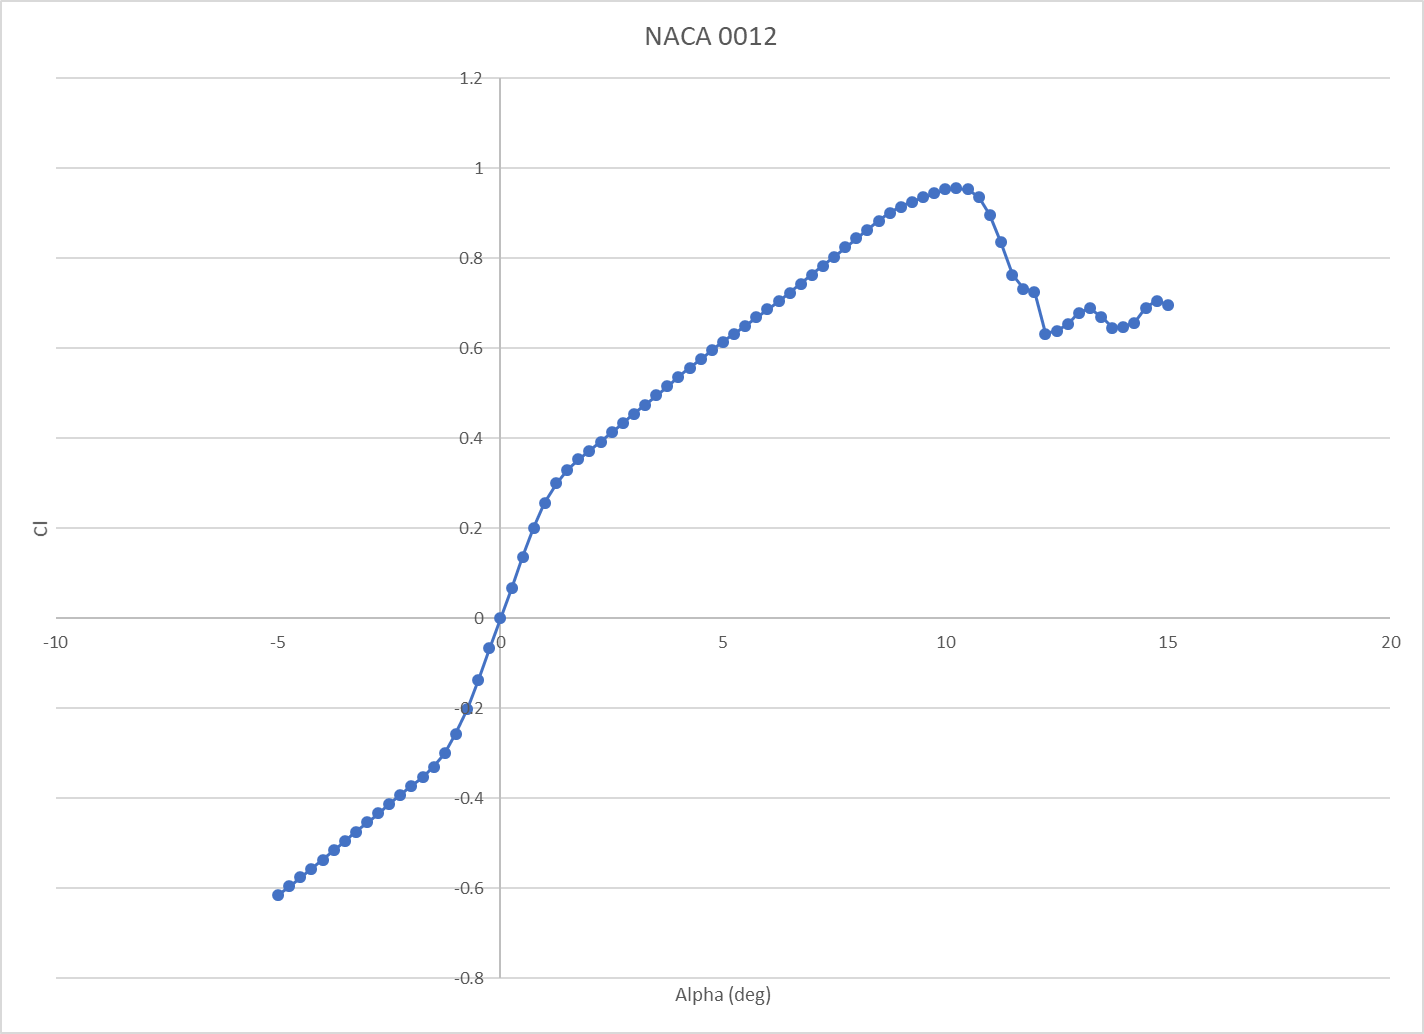
\includegraphics[scale=0.4]{NACA0012clvsalpha.png}
	\caption{NACA 0012 $Cl$ vs $\alpha$}
	\label{Figure 1:}

\end{center}
\end{figure}

\begin{figure}
\begin{center}
	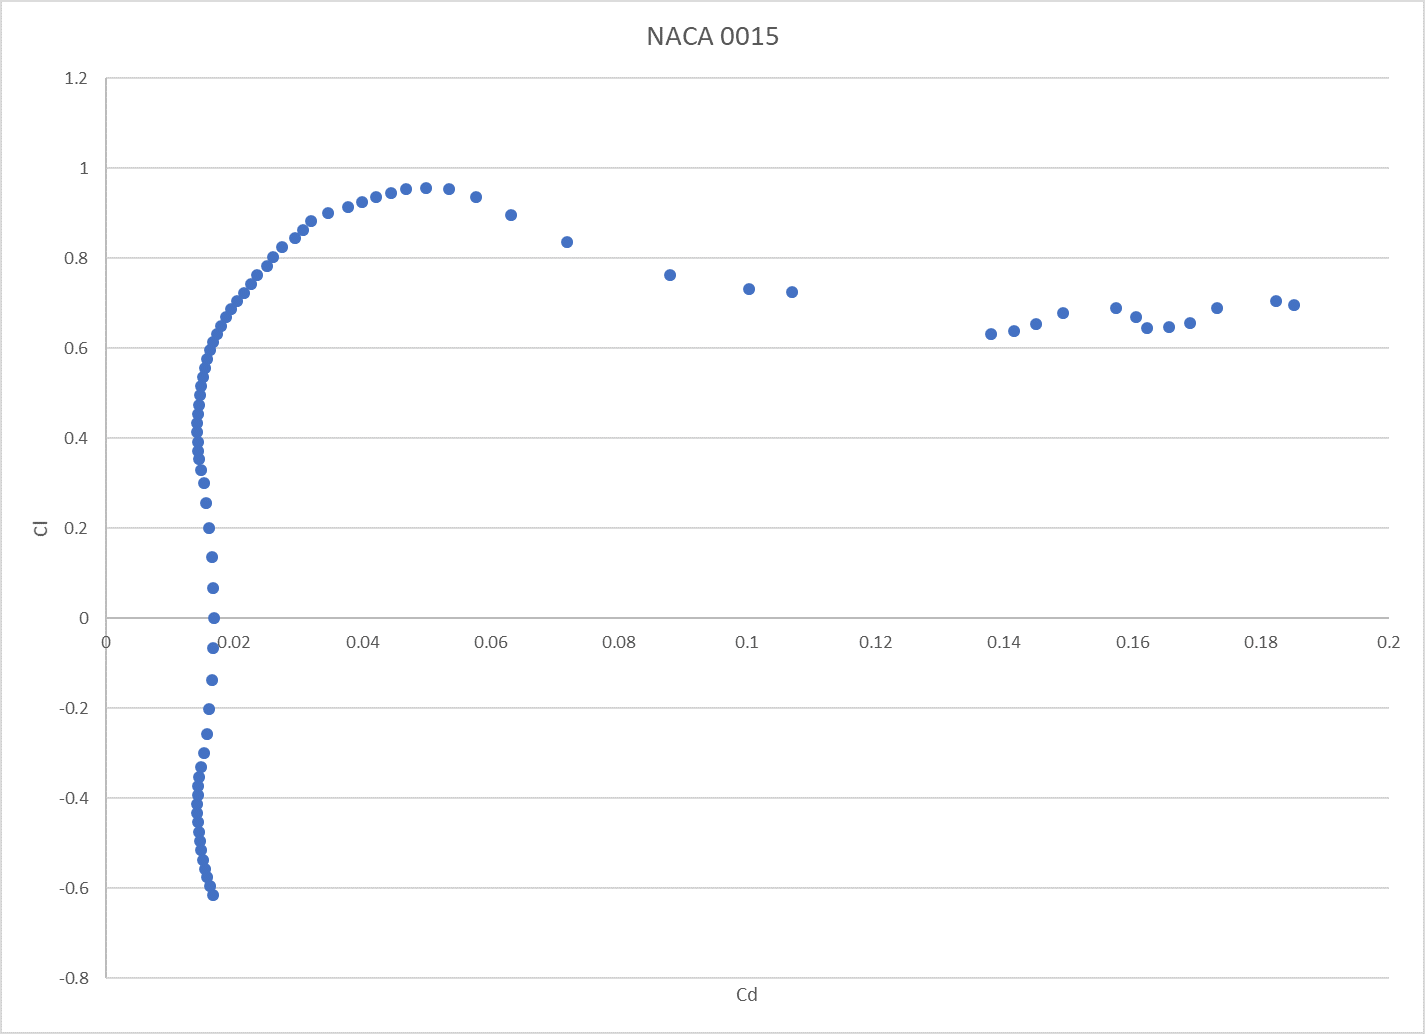
\includegraphics[scale=0.4]{NACA0012clvscd.png}
	\caption{NACA 0012 $Cl$ vs $Cd$}
	\label{Figure 1:}

\end{center}
\end{figure}

\section*{References}

[1] Anderson, J.D. (1999). Design of a Propeller-Driven Airplane. In K.T. Kane (Ed.), \textit{Aircraft Perfomance and Design} (pp. 433-440). United States of America: McGraw-Hill \\

\noindent [2] Sarker, Md. S., Panday, S., Rasel, Md., Salam, Md. A., Faisal, Kh. Md., \&  Farabi, T.H. (2017). Detail design of empennage of an unmanned aerial vehicle. \textit{AIP Conference Proceedings, 1919}(1), pp. 020033. doi: 10.1063/1.5018551\\

\noindent [3] Raymer, D.P. (1992). \textit{Aircraft Design: A Conceptual Approach}. Washington: American Institute of Aeronautics and Astronautics.






\end{document}